\documentclass{article}
\usepackage{preamble}


\begin{document}

\maketitle

\pagebreak

\section{Abstract}
In the current revolution of artificial intelligence, many companies are racing to create autonomous navigation and steering control algorithms for their vehicles. These software are made to handle various real-life scenarios such as obstacle avoidance and lane maneuvering. There are currently multiple researchers working on approaches to incorporate pothole avoidance into these autonomous systems using various different methods. However, there is very little research on the effect of hitting a pothole on the autonomous navigation software that is still using the camera to make driving decisions. This software must be made resilient against such perturbations in camera angle such that hitting a pothole in the car does not cause the predicted steering angle response of the autonomous control system to differ wildly from the proper steering response. This paper proposes a method for increasing robustness in steering control prediction algorithms by justifying a distribution of perturbations in camera angle caused by the average pothole and then using an AutoEncoder to simulate such perturbations repeatedly until the steering angle prediction model becomes resilient to the pothole interaction. When trained and tested, the model successfully became more robust based on the AMAI (Average, Mean Average, and Improvement) loss metric, meaning that this approach can successfully increase robustness in an autonomous control model against the dash cam image angle perturbations induced when one wheel of a car goes over a pothole.

\section{Introduction}

Cars have now become an integral piece of an American's lifestyle, with the average American now driving 14,263 miles per year, according to the Federal Highway Administration. Since American drivers now drive 3.2 trillion miles annually, there is a much greater need for emphasis on roadway safety~\cite{meyer_2023}. One commonly-overlooked danger is deteriorating road conditions leading to the formation of potholes. While most drivers consider them a minor nuisance that makes their drive less comfortable or a minor obstacle on the road to be avoided, potholes can actually have a dangerously significant impact on a vehicle. Direct contact with a pothole could result in an impact that causes injury, major damage to the vehicle, or even a result equivalent to that of a 35 mph vehicular crash~\cite{bodden_2021}. This is not even an uncommon problem, with \$26 billion being spent by drivers in 2021 to pay for pothole repair, and with 1 in 10 drivers needing to repair their vehicle after hitting a pothole~\cite{edmonds_2022}. 

In 2023, many automotive companies are now releasing their cars with novel steering assist systems or even full self-driving software, in the case of Tesla. While they can handle simple situations with other vehicles such as managing the car during a stop-and-go traffic jam, these autonomous navigation systems have not yet been adapted to the problem of avoiding potholes on the road. These systems will simply drive at full speed without adjusting the steering angle (the degree to which the steering wheel of the car is rotated) over a pothole as if it does not exist, which can be extremely dangerous if an inattentive driver fails to take control and correct the car's trajectory before the impact.

As more features get developed for these autonomous navigation systems, it is becoming crucial to address the issue of pothole avoidance in these systems, but it is also critical to predict a car's response to driving over a pothole. While some systems have been proposed for the avoidance of the pothole, there has been no working model proposed to determine the car's response to collision with the pothole. It is important to consider the consequences of a pothole impact and to regulate its effect on the car's autonomous navigation systems to maintain a safe response to the impact and keep the driver as far as possible from harm.

This paper will investigate approaches to minimize the consequences of a car's automatic response to a pothole collision by increasing the robustness of the autonomous navigation system in the car against the image perturbations (any deviation made to the image to change it from the original image, e.g. rotation in dash cam image angle) that result from such a collision, which will normalize the car's predicted steering angle response and remove any extraneous predictions post-collision even in the face of such image perturbations.

\section{Related works}

Multiple researchers have attempted to solve the problem of corrective obstacle avoidance. In these methods, the avoidance logic can be easily extended to potholes in the road such that the autonomous navigation model will turn the steering wheel accordingly to avoid the incoming pothole on the road. The researchers have proposed different approaches that can broadly be categorized into one of three categories: vibration-based, depth-based, and GPS-based approaches.


\subsection{Vibration-Based Approach}

Some approaches have been formulated that use sensors such as speedometers and accelerometers to identify and classify the potholes with vehicle encounters. They do this by mathematically modeling the jerk induced by traveling over a pothole on the car’s suspension, and then analyzing the sensor input by feeding it into a Bayes decision classifier to record the proper response from hitting the pothole. These approaches are fairly accurate in identifying when the vehicle encounters a pothole, but due to the limited reaction time of a vehicle, there is very little the algorithm can do to actually avoid the pothole other than know when it is encountered in real-time. There is also very little the algorithm can do in terms of reacting to the information being provided at the moment due to limited processing time and sensor limitations. The reason for this is that the approach can only formulate a reaction to the pothole once it detects it with the vibrations in the car, at which point it is too late to react properly. While this may be a useful aspect of the pothole collision problem by accurately recording the resulting discomfort levels of hitting a pothole, it cannot solve the initial pothole avoidance problem in its entirety~\cite{li2015road}.

\subsection{Depth-Based Approach}

 To help flush out the limitations of the vibration-based pothole avoidance approaches, other researchers have proposed a depth-based pothole mapping system that can use recorded data from LiDAR sensors and the approximate distance of the surface to identify pavement anomalies. This approach is one of the most reliable at identifying information about the upcoming potholes ahead of time, but a LiDAR sensor is limited to only gathering information about the distance to the pavement in front of the car. For the car to perform reactive and corrective steering, it needs to be aware of its surroundings and make decisions based on inputs from its environment as well. This is the same issue seen in the vibration-based approach proposed by Z. Li~\cite{kang2017pothole}.

\subsection{GPS-Based Approach}

Finally, there have been numerous methods proposed to crowd-source the recording of potholes similar to collecting data for google maps. These approaches use sensors in the car to identify when it has passed over a pothole, then it records this data along with GPS coordinates and sends it to a central server. This information can then be used to warn other cars that are fitted with the same system of upcoming potholes. However, this means that the car can only react if another car has already gone over the pothole at full speed and recorded it, and if the pothole is patched or worsened, the car will not have updated information as it will simply avoid the area altogether. This may also lead to some privacy concerns with user GPS data being constantly monitored and transmitted through a third-party server, and this is overall not a feasible or viable real-time reactive approach or final solution~\cite{kamalesh2021intelligent,kulkarni2014pothole}.

\subsection{The Gap}

Each of these three approaches utilizes a different strategy to predict the correct reaction to a pothole encounter. Li, Zhaojian et al.~\cite{li2015road} analyze the impact of the pothole on the car mid-collision, while Byeong-ho Kang et al.~\cite{kang2017pothole} use computer vision to classify and identify the pothole prior to it encountering the car. MS Kamalesh~\cite{kamalesh2021intelligent} and Aniket Kulkarni~\cite{kulkarni2014pothole} propose GPS-based approaches that can identify the pothole well in advance, but cannot give information to the self-driving system until one car goes over the pothole and does not have real-time information about the road situation around it. While there is much development being made on these different strategies to handle the moments prior to the encounter, there is very little research about the post-impact effects on the autonomous navigation system. 

Therefore, the purpose of this research is to develop a technique for increasing the robustness of steering control algorithms in response to perturbations due to the impact of a car with a pothole.

\section{Method}

The most effective way to answer this project's guiding research question is to perform real-world testing by attaching a camera to a car and testing various algorithms in the car when driven over potholes. However, for the scope of this project, it is more feasible and practical to simulate the effect of such a real-world experiment in a simulation that uses some basic assumptions that can be fine-tuned to any car or situation this method is to be adapted to in a real-world experiment.

\subsection{Pothole Generation}

The first step in analyzing the effects of a pothole collision is to establish what the potholes themselves look like. There is a wide variety of potholes on the roads and the range of possible potholes to encounter is very large. In order to represent the average pothole collision, we must first take a sample of various potholes on an average roadway. To do this, I have utilized a publicly available dataset that incorporates novel algorithms for road disparity (or inverse depth) transformation, deployed on a semantic segmentation network. This means that the researchers have developed a technique to use multiple stereo cameras positioned at varying angles on a moving car to capture 3-D visualizations of damage in roadways along with RGB overlays (color images) of the same damaged areas. 

This dataset includes 600 samples of potholes split into 180 samples in a testing group, 240 samples in a training group, and 180 samples in a validation group. This ratio of images split into multiple groups is commonly used in machine learning applications, but since this research will only be using this dataset to represent a sample of all potholes in roadways, we proceed by combining all samples into one group of 600 potholes. This group contains an RGB color image (e.g. Figure \ref{fig:potholeimagergb}), a heatmap in the jet color scale (e.g. Figure \ref{fig:potholeimagetdisp}), and a strictly black and white label image (e.g. Figure \ref{fig:potholeimagelabel}). The heatmap uses the jet color scale because it is the default output color scale in the Matlab programming language, which is the language of choice for Fan, R. et al. to show a displacement map of the pothole (indicating areas of low depth with the color blue and areas of high depths with the color red) in the road for each of the 600 images~\cite{8300645, 8809907, 8890001}.


\begin{figure}[!htb]
    \minipage{0.32\textwidth}
        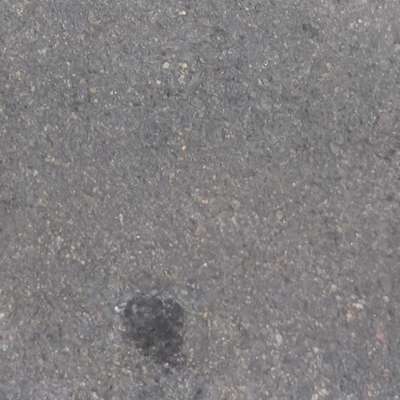
\includegraphics[width=\linewidth]{0000rgb.png}
        \caption{RGB scan of top-down view for a sample pothole}\label{fig:potholeimagergb}
    \endminipage\hfill
    \minipage{0.32\textwidth}
        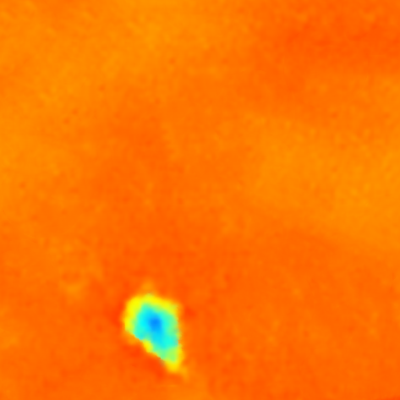
\includegraphics[width=\linewidth]{0000tdisp.png}
        \caption{Jet colorscale heatmap of depth for a sample pothole}\label{fig:potholeimagetdisp}
    \endminipage\hfill
    \minipage{0.32\textwidth}%
        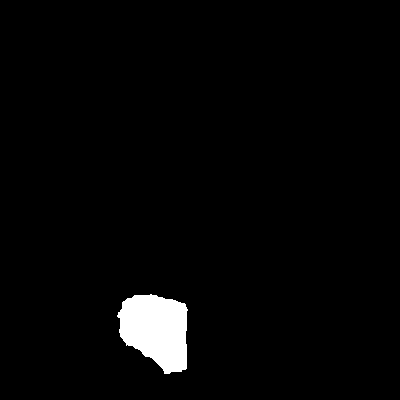
\includegraphics[width=\linewidth]{0000label.png}
        \caption{Strictly black-and-white label image for a sample pothole}\label{fig:potholeimagelabel}
    \endminipage
\end{figure}


In order to proceed with performing an analysis of this collection of potholes, they must first be combined into 3-D representations of potholes that can then be statistically analyzed to extract various average measurements of the potholes, and these measurements can then be used with measurements from accurate car diagrams to determine the effect of driving over the pothole on a car and its camera.

The program of choice for this 3-D reconstruction is known as Blender, which is a free and open-source powerful 3-D modeling software used by multiple different industries for different parts of the 3-D pipeline, such as modeling, sculpting, visual effects, computer graphics, UV Unwrapping, virtual reality, and even creating fully animated films. 


Since there are 600 different potholes, it would be a lengthy process to individually combine the three images into a 3-D model for each of the samples. Coincidentally, Blender implemented a new Python API in Blender 2.5, developed from 2009 to August 2011~\cite{blendermanual_2022}. This Python API allows for the interaction between the Python programming language and the Blender software, which is an extremely powerful integration considering the versatility of the Python programming language. 

I proceeded by creating a Blender script in Python (Listing \ref{code:blender}) to take each of the 1800 images (600 groups of 3 images) and recursively process each of them into a complete 3-D file. Automating this process likely saved up to weeks of mundane and repetitive work.

\begin{code}
\captionof{listing}{Source code for Blender pothole generation script in Python \cite{blender_2022}}
\label{code:blender}
\begin{minted}{python}
# Package imports
import bpy
import os

# Source image path
path = "C:\\Users\\shiva\\Downloads\\pothole600\\blender\\source_images"

# Iterate over each source image
for pothole in os.listdir(path):

        # Open each source image and define relative paths to all other parts of the same model
        for image in os.listdir(f"{path}\\{pothole}"):
        bpy.ops.image.open(
            filepath=f"//..\\..\\..\\..\\Downloads\\pothole600\\blender"
                     f"\\source_images\\{pothole}\\{image}",
            directory=f"C:\\Users\\shiva\\Downloads\\pothole600\\blender"
                      f"\\source_images\\{pothole}\\")

    # Add plane
    bpy.ops.mesh.primitive_plane_add()
    so = bpy.context.active_object

    # Add subdivision surface modifier to add malleable detail to the plane
    mod_subsurf = so.modifiers.new("subdivision", "SUBSURF")
    mod_subsurf.levels = 7
    mod_subsurf.render_levels = 7

    # Add displacement modifier to handle displacement using the heatmap as a displacement texture
    mod_displace = so.modifiers.new("displacement", "DISPLACE")
    mod_displace.strength = -1
    disp_texture = bpy.data.textures.new("tdisp", "IMAGE")
    disp_texture.image = bpy.data.images["tdisp.png"]
    mod_displace.texture = disp_texture

    # Create a material to be assigned to the model
    pothole_material = bpy.data.materials.new(name="rgb")

    # Set up tree nodes to implement material
    pothole_material.use_nodes = True
    nodes = pothole_material.node_tree.nodes

    # Procedurally assign material to the object using nodes
    bsdf = nodes["Principled BSDF"]
    texImage = nodes.new('ShaderNodeTexImage')
    texImage.image = bpy.data.images["rgb.png"]
    pothole_material.node_tree.links.new(bsdf.inputs['Base Color'], texImage.outputs['Color'])

    so.data.materials.append(pothole_material)

    # Shade smooth
    bpy.ops.object.shade_smooth()
    
    # Export
    # fbx was chosen as the export file format for direct Unreal Engine imports and integration
    bpy.ops.export_scene.fbx(filepath=f"C:\\Users\\shiva\\Downloads"
                                      f"\\pothole600\\blender"
                                      f"\\potholes\\{pothole}.fbx")

    # Delete all previous objects
    bpy.ops.object.select_all(action='SELECT')
    bpy.ops.object.delete(use_global=False, confirm=False)

    print(pothole)

    # Delete all previous textures
    for texture in bpy.data.textures.values():
        bpy.data.textures.remove(texture)

    # Delete all previous materials
    for material in bpy.data.materials.values():
        bpy.data.materials.remove(material)

    # Delete all previous images
    for image in bpy.data.images.values():
        bpy.data.images.remove(image)
    
    # Blender workspace is now completely clear and ready to process the next set of pothole images
\end{minted}
\end{code}

\begin{figure}[h!]
    \centering
    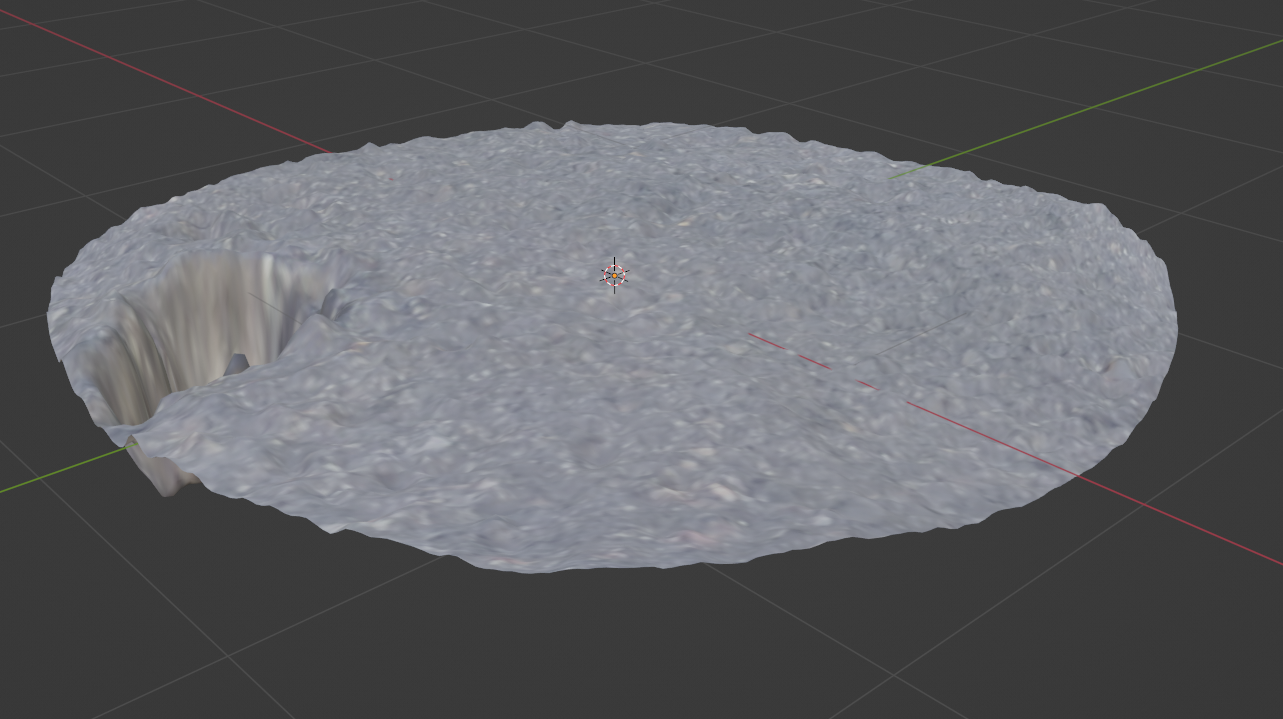
\includegraphics[width=\textwidth]{pothole3D.png}
    \caption{3-D Object created by the program in Listing 1 for a sample pothole}
    \label{fig:pothole3D}
\end{figure}

\subsection{Image Perturbations}

Now that we have a collection of 600 physical models of potholes, the next step is to perform a statistical analysis of those potholes. The approach taken to do this will be a separate, standalone Python program that will process all of the 3-D objects created by the Blender program. This Python program imports each 3-D project and then saves a matrix of gradients for every point on the model, essentially creating a dataset of slopes (rate of change in depth of the pothole) for every pixel of the model. Then, the program discretizes this matrix into a 10 by 10 set of equally-sized squares, giving us 100 different small portions of the pothole. We then take the average gradient for each of the 100 squares (taking the direction of each of the slopes into account) and save this as the new matrix representing the model of the pothole. The reason we do this is to reduce the amount of data that is needed to represent the pothole, which makes it much easier and faster to process.

After the program repeats the pothole modeling process for each of the 600 models, it saves the 10 by 10 matrix of average gradients of each pothole into one big dataset containing 60,000 values representing each of the potholes. At this point, we have successfully turned the entire set of 3-D pothole models into a low-level representative dataset of numerical values, on which we can then perform a statistical analysis to obtain average statistics and measures of variability and central tendency in the sample of potholes.

\begin{code}
\captionof{listing}{Standalone Python script for statistical 3-D Pothole analysis}
\label{code:blender}
\begin{minted}{python}
# Package imports
from PIL import Image
import numpy as np
import os
import pandas as pd

# Store the average image gradients from each chunk for each image
allImageGrads = []

# Open and recursively process all 3-D pothole objects
for file in os.listdir("pothole600/pothole600/"):
    if file.endswith(".fbx"):

        # Open each 3-D object as a numpy array to be easily processed
        imNP = np.array(open("pothole600/pothole600/" + file))

        # Split image into chunks of 40 (10, 10, 40, 40, 3)
        # 10 rows, 10 columns, 40x40 pixels, 3 color channels
        imageArray = np.zeros((10, 10, 40, 40, 3))
        for rowNum in range(10):
            for colNum in range(10):
                imageArray[rowNum, colNum] = imNP[rowNum*40:(rowNum+1)*40, colNum*40:(colNum+1)*40, :]
        # imageArray now contains 10x10 chunks of 40x40 pixels for 3 color channels

        # Find the average gradient of each chunk
        grads = []
        split_array = cubify(imNP, (40, 40, 3))
        for i in range(10):
            for j in range(10):
                cube = split_array[i, j]
                cube_values = []
                grads.append(np.argmax(np.gradient(cube)))

                sumChannels = []
                for k in range(40):
                    sumChannels.append(np.gradient(int(sum(cube[k]) / 3)))

        # Add the average of all 100 gradients in the pothole to the overarching list containing all average gradient values, one for each pothole
        allImageGrads.append(np.average(grads))

# Print the pandas statistical analysis on the obtained average gradients for all potholes
pdSeries = pd.Series(allImageGrads)
print(pdSeries.describe())
\end{minted}
\end{code}

\begin{table}[h!]
\centering
\begin{tabular}{||c | c||} 
 \hline
 Statistic & Value (mm)\\  
 \hline\hline
 count & 600.000000\\ 
 \hline
 mean & 61.724417\\
 \hline
 std & 10.208508\\
 \hline
 min & 47.450000\\
 \hline
 25\% & 55.812500\\ 
 \hline
 50\% & 59.490000\\ 
 \hline
 75\% & 63.862500\\ 
 \hline
 max & 108.500000\\ 
 \hline
 \end{tabular}
 \caption{Statistical output from Listing \ref{code:blender}}
 \label{table:potholestats}
\end{table}


Now that we have the average statistical values that represent potholes, we must now find the most representative method for using them in our simulation. The approach for this will be to analyze the physical construction of the typical vehicle and treat it as a rigid body, then calculate the effect of hitting the average pothole on the image input from a dash cam mounted facing the front of the car that is being used for autonomous navigation. In order to do this, some basic assumptions about the dimensions of the average car must be made.

In 2022, the best-selling passenger car worldwide was the Toyota Corolla, acquiring 1.12 million sales~\cite{carstats}. Therefore, we will be using the Toyota Corolla to represent our average, everyday car driving on the roadways. 

\begin{figure}[h!]
    \centering
    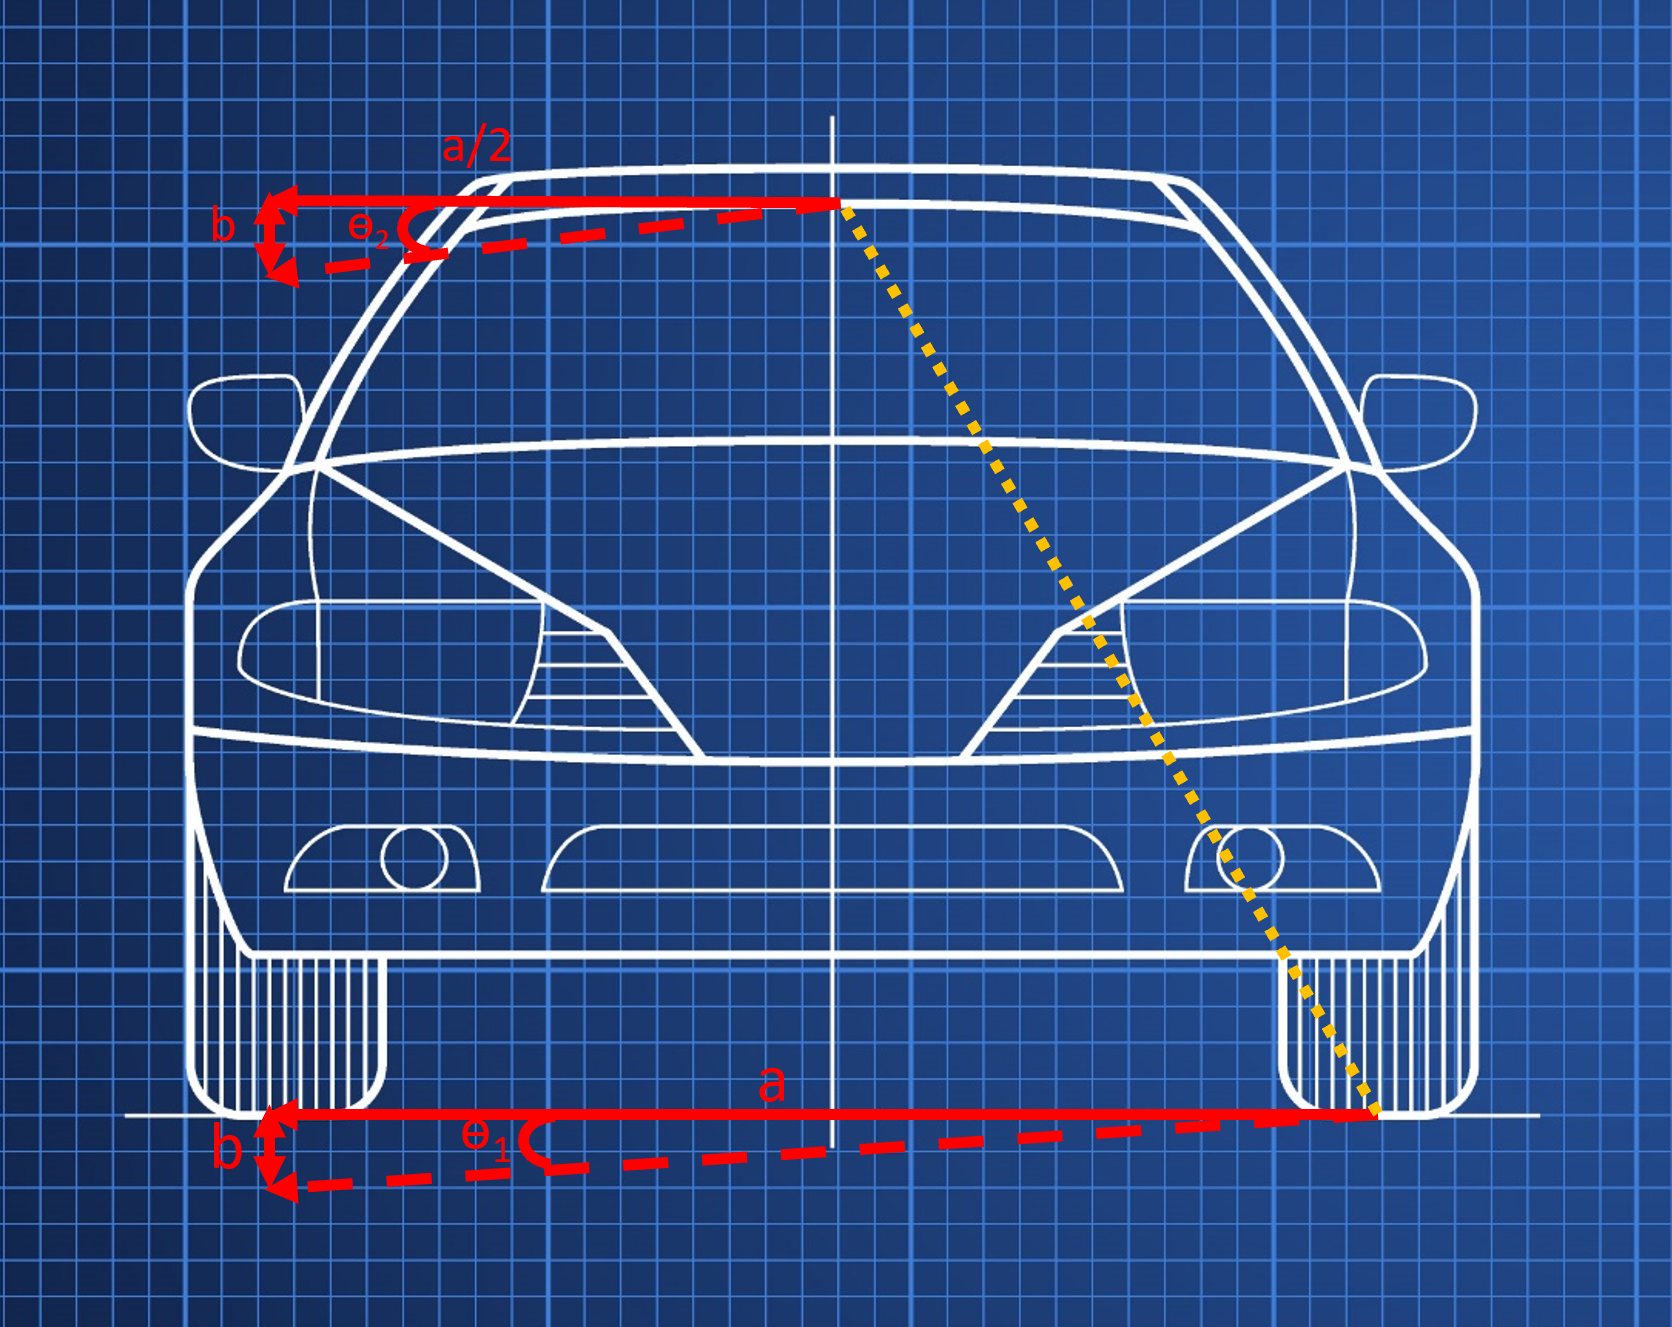
\includegraphics[width=\textwidth]{cardiagram.png}
    \caption{Diagram representing a typical pothole collision with a car \cite{cardiagram}}
    \label{fig:cardiagram}
\end{figure}

In Figure~\ref{fig:cardiagram}, $a$ represents the width of the car from the middle of each wheel. This will be estimated using the baseline assumption of the Toyota Corolla, which has a width of 1780 mm (1.78 m). The letter $b$ represents the amount that the wheel dips down due to a pothole impact. For the purposes of this research, we will assume that the car is a rigid body because accounting for suspension in our calculations would be out of the scope of this project. Therefore, we can simply use the sample distribution of pothole depths given by our statistical analysis of the pothole models and directly plug them into b to get the offset of the car. After that information is plugged in, we need only to perform some trigonometry to obtain our distribution of angles $\theta_2$ that represents the average dash cam perturbation in terms of the angle by which the image is shifted.

\begin{align*}
\label{eqn:potholeangles}
    a = 1780 mm \\
    b \approx 61.72 mm \\
    \tan\theta_1&= \frac{b}{a} \\
    \theta_1&= \arctan\frac{b}{a} \\
    \theta_2&= \arctan\frac{2b}{a} \\
    \theta_2&= \arctan\frac{123.44}{1780} \\
    \theta_2&\approx 0.0692 \cdot \frac{180}{\pi} \\
    &= 3.967\degree
\tag{Derivation 1}
\end{align*}
\ref{eqn:potholeangles} outlines sample mathematical steps used to convert pothole depths to camera angle perturbations.

Now, we simply perform the steps in~\ref{eqn:potholeangles} on the distribution of pothole angle depths outlined in Table~\ref{table:potholestats} to obtain a justified and statistically sound distribution of angle perturbations to dash cam images. Then, it is time to perform the simulation of the effect such perturbations will have on autonomous navigation systems and to develop a steering-angle prediction model that becomes resilient against those perturbations within the simulation.

For the simulation itself, this project will utilize a custom-built and modified version of the AutoJoin AutoEncoder, outlined by Michael Villarreal, with dash cam perturbations only relevant to pothole interactions~\cite{villarreal2022autojoin}. The primary edits made for the purposes of this research project are that I have gone in and edited the tested perturbations by removing the ones irrelevant to the topic of this research and adding perturbations that were generated by the method outlined in this project. After doing so, and adapting the rest of the code to work with the new set of perturbations, we are ready to run the autoencoder.

The basic concept of an autoencoder is to reduce input images to a low-dimensional representation (essentially a blurry image with much less information and detail) and then train the machine learning model to recreate the original image from that low-dimensional representation. Since the model can now recreate an image from one containing less data, this technique is commonly used in denoisers to add detail to an image, but in the case of AutoJoin, it is implemented to increase the robustness of an existing autonomous navigation system against noise in dash cam footage.

For this research, we will be using a dataset of dash cam images provided by Audi and Honda, which has about 850,000 training, testing, and validation images. We then apply the distribution of angle perturbations to the training images in this dataset to generate the perturbed training images. For this research, we will be using the NVIDIA autonomous navigation model (a pre-made neural network created by NVIDIA to take an input dash cam image and return a predicted steering angle) for steering angle prediction. When we run the autoencoder, the pre-built model will be fed the original dash cam image first, and the predicted steering angle will be taken as the ground truth or actual correct steering angle in normal conditions. Then, a perturbed dash cam image (as if the car is currently going over a pothole) will be fed into the model, and the difference in the predicted output steering angle for the two images (the ground truth steering angle and the perturbed image steering angle) will be calculated. Then, the autoencoder is trained to reduce the noise in the perturbed image and introduce bias in the model such that the difference between the actual steering angle and the steering angle predicted by the pre-trained model on the perturbed dash cam image is minimized until the model gets as close as possible to the original output even on a perturbed image. Once this happens, the self-driving algorithm has essentially become robust against the image perturbation we have introduced, and will not be nearly as severely affected by the change in dash cam angle introduced when a car is driven over a pothole.

This autoencoder was trained and tested on about 500,000 images for 50 epochs (meaning that it goes over each image 50 times when relearning the correct model output). Since there is such a large amount of data processing happening at once, the individual matrix calculations (the mathematical explanation for what happens behind the scenes when a computer processes and manipulates an image) performed during the testing and especially training phases of this model will be performed on a desktop computer with 32 gigabytes of RAM and an NVIDIA GeForce RTX 3090, which has Tensor cores optimized for processing the large matrices associated with this model training process. The whole program still takes over 12 hours, even with such a high-power PC continuously running at its highest performance setting.

\section{Results}

In order to evaluate the performance of the model on the perturbations, we make use of the AMAI metric. This evaluation metric utilizes three combined factors: Average, Mean Accuracy, and Improvement values.

\subsection{Average Factor}

The average factor is the average predicted steering angle obtained by the model over all test perturbations within our dash cam category.

\subsection{Mean Accuracy Factor}

The mean accuracy is a percentage value obtained by comparing the differences between predicted and actual steering angles (by giving perturbed and original images as inputs to feed into the model) over 5 threshold values. Since the steering angle is a continuous value, we use threshold values to determine how close the prediction angle is to the actual (or ground truth) angle.

The mean accuracy metric is used specifically to bridge a gap that exists between using continuous values and discrete outputs to evaluate the performance of a model. With discrete classifications, it is simple to determine whether two outputs fall into the same category. With a continuous output, however, we use the threshold values to establish a range of acceptable steering angles that will be considered a success for the model if it obtains an output within that range.

\subsection{Improvement Factor}

And finally, the improvement metric is the difference between the robust model's performance and a standard/baseline model's performance (this standard model is trained only on the original clean images using the same architecture as the robust models) within a test category. This metric will help incorporate the amount of robustness that the new model has acquired over the original model and primarily determines how successful the overall training and testing process of the autoencoder has been.

\subsection{AMAI Model Loss}

These three metrics are combined into the AMAI loss metric, which we will be using to evaluate the performance of our model. We can see from Table 2 that the Overall AMAI and the Unseen Perturb column, which is the primary indicator of the improvement of the model, all decrease consistently over time throughout the rows of the column. 

\begin{table}[h!]
\centering
\begin{tabular}{||c c c c||} 
 \hline
 \multicolumn{4}{|c|}{Overall AMAI: 68.00175621052631} \\ [0.5ex]
 \hline\hline
  Clean & Single Perturb & Combined Perturb & Unseen Perturb \\ [0.5ex] 
  \hline\hline
 67.02 & 65.75 & 63.37 & 68.50 \\ 
 \hline
 
 \hline
 \multicolumn{4}{|c|}{Overall AMAI: 23.567438017694574} \\ [0.5ex]
 \hline\hline
  Clean & Single Perturb & Combined Perturb & Unseen Perturb \\ [0.5ex] 
  \hline\hline
 24.99 & 25.09 & 25.44 & 23.24 \\ 
 \hline

  \hline
 \multicolumn{4}{|c|}{Overall AMAI: 10.706730520097834} \\ [0.5ex]
 \hline\hline
  Clean & Single Perturb & Combined Perturb & Unseen Perturb \\ [0.5ex] 
  \hline\hline
 11.55 & 11.76 & 12.43 & 10.48 \\ 
 \hline
\end{tabular}
\label{table:AMAIlosses}
\caption{This table shows the AMAI losses for different categories obtained by the model}
\end{table}

Now that the model has been tested and its AMAI loss has been obtained, we can proceed to analyze the change in the loss over time after each epoch. The most effective way to do so is to graph the loss over the number of epochs, giving a visual demonstration of the decrease in loss over time, which indicates a model that has been successfully trained.

From Figure 6, we can see that the overall AMAI loss decreases over time as the model is trained for longer and on more data, and we can see that the average loss decreases and approaches zero during the testing phase in Figure 7, meaning that our model has successfully become resistant to perturbations in camera angle due to collisions with potholes.

\begin{figure}[h]
    \centering
    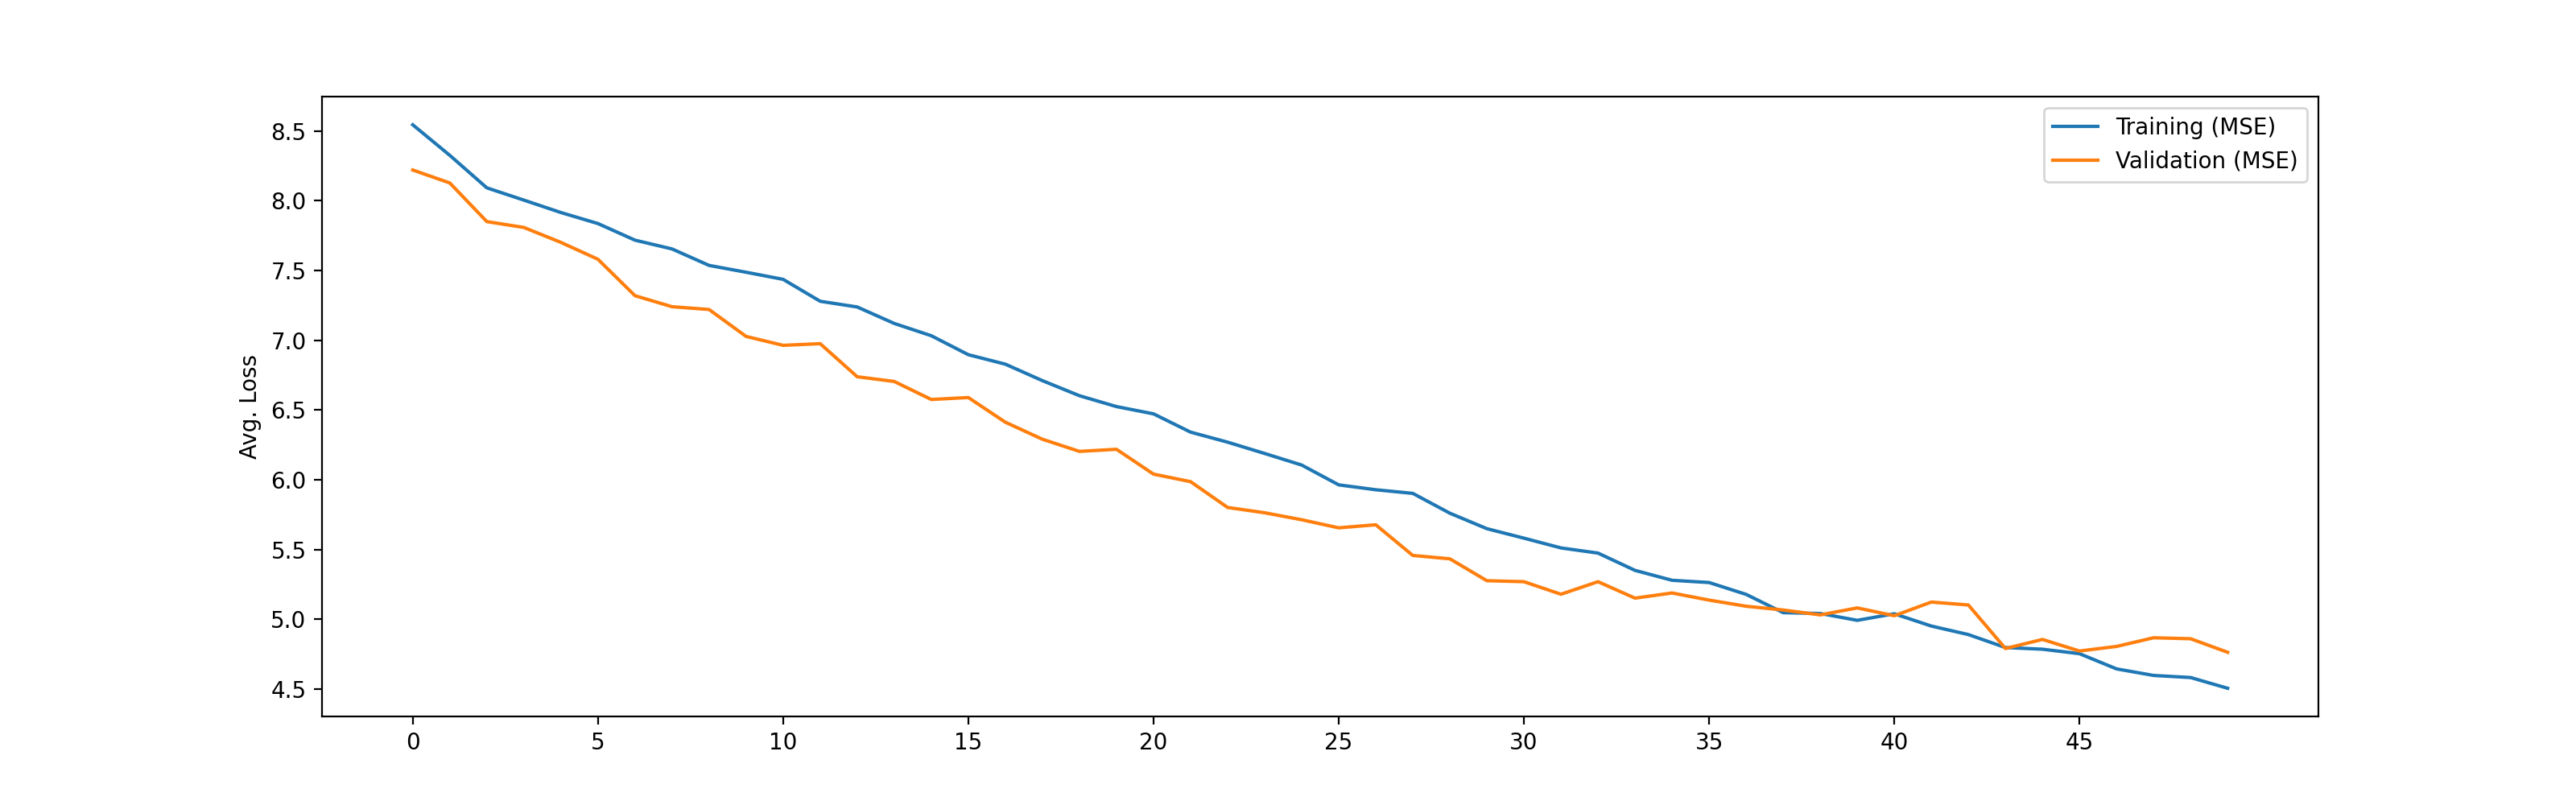
\includegraphics[width=\textwidth]{training_graph_reg.png}
    \label{fig:traingraph}
    \caption{Graph of change in loss over time during the training phase}
\end{figure}
\begin{figure}[h]
    \centering
    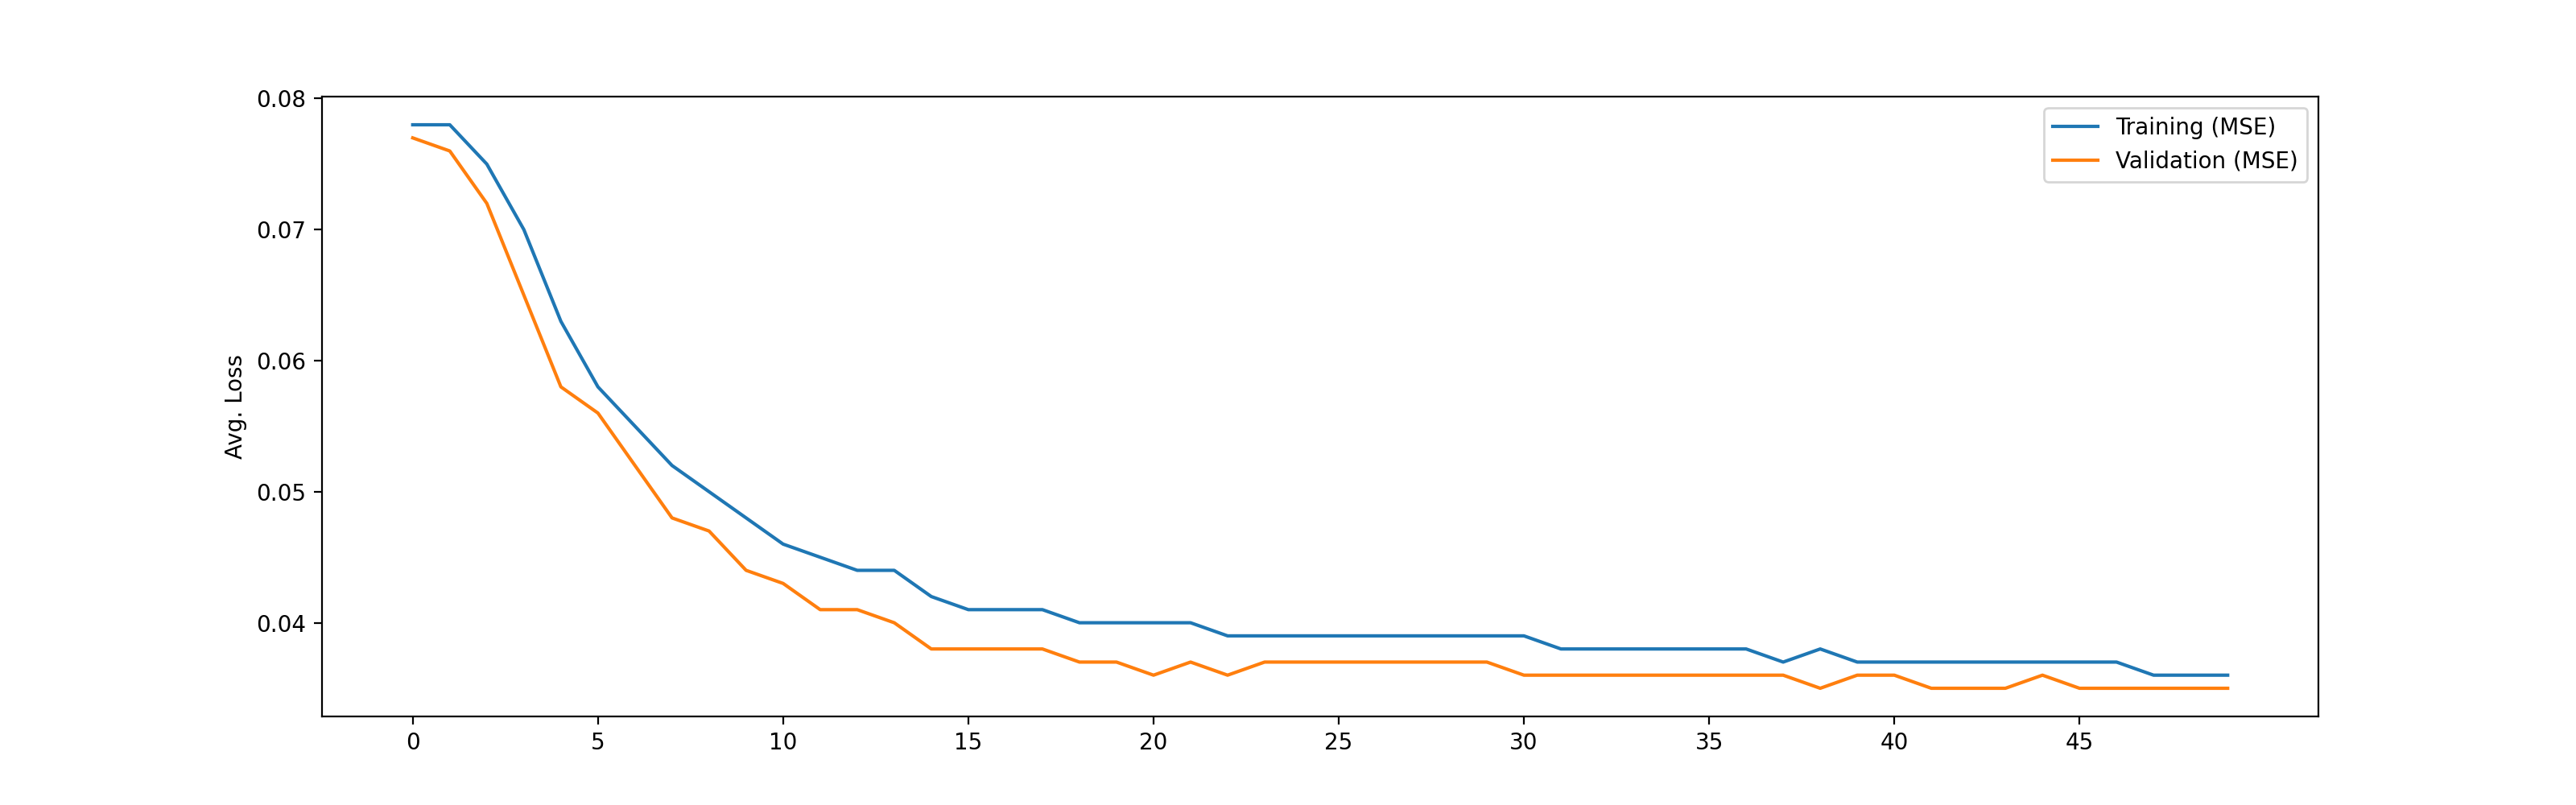
\includegraphics[width=\textwidth]{training_graph_recon.png}
    \label{fig:testgraph}
    \caption{Graph of change in loss over time during the testing phase}
\end{figure}

\newpage

\section{Conclusion}

The goal of this research paper was to develop a method for creating robustness in an autonomous navigation algorithm to be resilient to perturbations associated with pothole collisions. As seen by the analysis in the results section, the chosen autonomous navigation algorithm was made greatly more resistant to the pothole image perturbations, and the perturbations themselves have been scientifically justified by performing sample analysis to get a statistical distribution of the perturbations. Therefore, within the scope of this project, we have successfully provided an answer to the guiding research question considering a method to increase the robustness of autonomous navigation systems based on computer vision against perturbations in camera angle due to collisions with potholes.

This research can begin to address the gap that currently exists in considering the immediate effects of a pothole encounter. While many researchers have attacked the problem of avoiding the pothole in the first place, certain systems, such as the depth-based approaches described in section 3.2, could greatly benefit from having a second system that consists of robust self-driving software as a failsafe in case that method is not able to successfully detect or avoid the pothole. This cooperation between approaches would introduce a redundancy in the self-driving pipeline which is almost always a necessity for a well-working engineering solution. This robustness approach can be combined with virtually any of the methods described in section 3 by simply adding the robust model at the end of the pre-existing self-driving model, meaning that the approach proposed in this paper can cooperatively interact with any of the researchers' papers to build on their solution.

There were many assumptions made in this research that may limit the potential implications of our findings. The most major assumptions were made during the creation of the image perturbation distribution, such as when the car was assumed to be a Toyota Corolla and the car was treated as a rigid body with no suspension. This likely skewed our data to have harsher angles than there would be in real cars, but this was not enough to pose a risk of our model becoming overly resilient. In the real world, the car could be one of a very wide selection of self-driving vehicles and it will likely have a suspension of varying levels of effectiveness. This test is also based almost entirely on simulation, so the technique needs to be implemented in a physical car to test the true impact of the robust model in real-world scenarios. If this were to happen, the car wheelbase and the impact of suspension should be taken into account and incorporated into the experiment to obtain the most accurate results.

The initial pothole sample itself is also a limitation in that it is not a completely representative sample of all potholes, it is only the potholes that the ZED stereo camera was able to catch, so there may be other deformations in the road such as broken speedbumps or major dips that have a similar image perturbation effect on the dash cam footage but were not incorporated in the training of our robust model. While this may skew our results to be less or more severe depending on the frequency of alternative road deformations on the road being tested, since the overall effect on the camera is similar, the robust model should still be able to handle the perturbation despite not being trained and optimized to deal with the scenario.

This research could potentially be implemented in existing autonomous navigation systems as an additional feature, such as in Tesla's autopilot, without the need for any major restructuring of the preexisting self-driving model. This will become crucial as more and more companies begin to implement advanced adaptive steering control systems based on camera input.

This research can be expanded by investigating the effect of different road deformations such as speedbumps or different angles of collision with potholes (such as one pothole on each wheel) on the camera input for the self-driving model. This would help make this approach more thorough and would increase the practicality of real-world implementation, which is the most immediate future direction for further research on this project.


\pagebreak
\bibliographystyle{acm}
\bibliography{bibliography}

\end{document}
